%%%%% Description: three work in the 1+3-framework %%%%%
%%%%% Created: July 24, 2016 %%%%%
%%%%% Author: Hengfeng Wei (hengxin) %%%%%

\documentclass{standalone}

\usepackage{tikz}
\usetikzlibrary{positioning, shapes, shapes.geometric, backgrounds, fit, arrows.meta, calc}
\usepackage{varwidth}

\begin{document}
\begin{tikzpicture}[node distance = 0.00cm]
  \node (f) [opacity = 0.60, label = {[font = \tiny, yshift = 0.10cm, text opacity = 0.60] below : framework}] {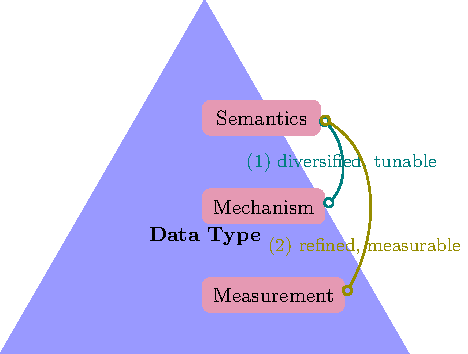
\includegraphics[scale = 0.15]{1+3-framework.pdf}};

  \node (vpc) [above = of f, label = {[font = \small, yshift = 0.10cm] below : (1) VPC}] {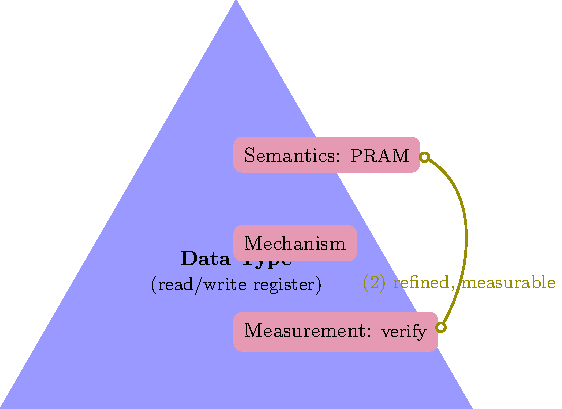
\includegraphics[scale = 0.30]{vpc-1+3-framework.pdf}};
  \node (pa2am) [right = of f.-30, xshift = -0.50cm, label = {[font = \small, yshift = 0.10cm] below : (2) PA2AM}] {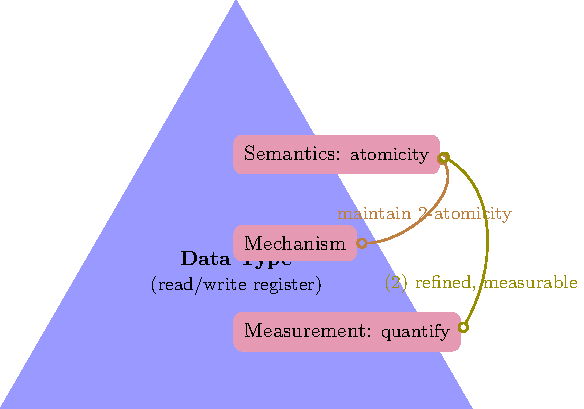
\includegraphics[scale = 0.30]{pa2am-1+3-framework.pdf}};
  \node (rvsi) [left = of f.-150, xshift = 0.50cm, label = {[font = \small, yshift = 0.10cm] below : (3) RVSI}] {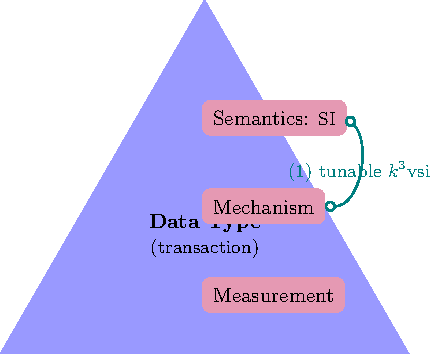
\includegraphics[scale = 0.35]{rvsi-1+3-framework.pdf}};
\end{tikzpicture}
\end{document}
